\begin{figure}[htbp]
\centering
\begin{tikzpicture}[x=1cm,y=1cm]
\node[anchor=south west,inner sep=0] at (0,0) {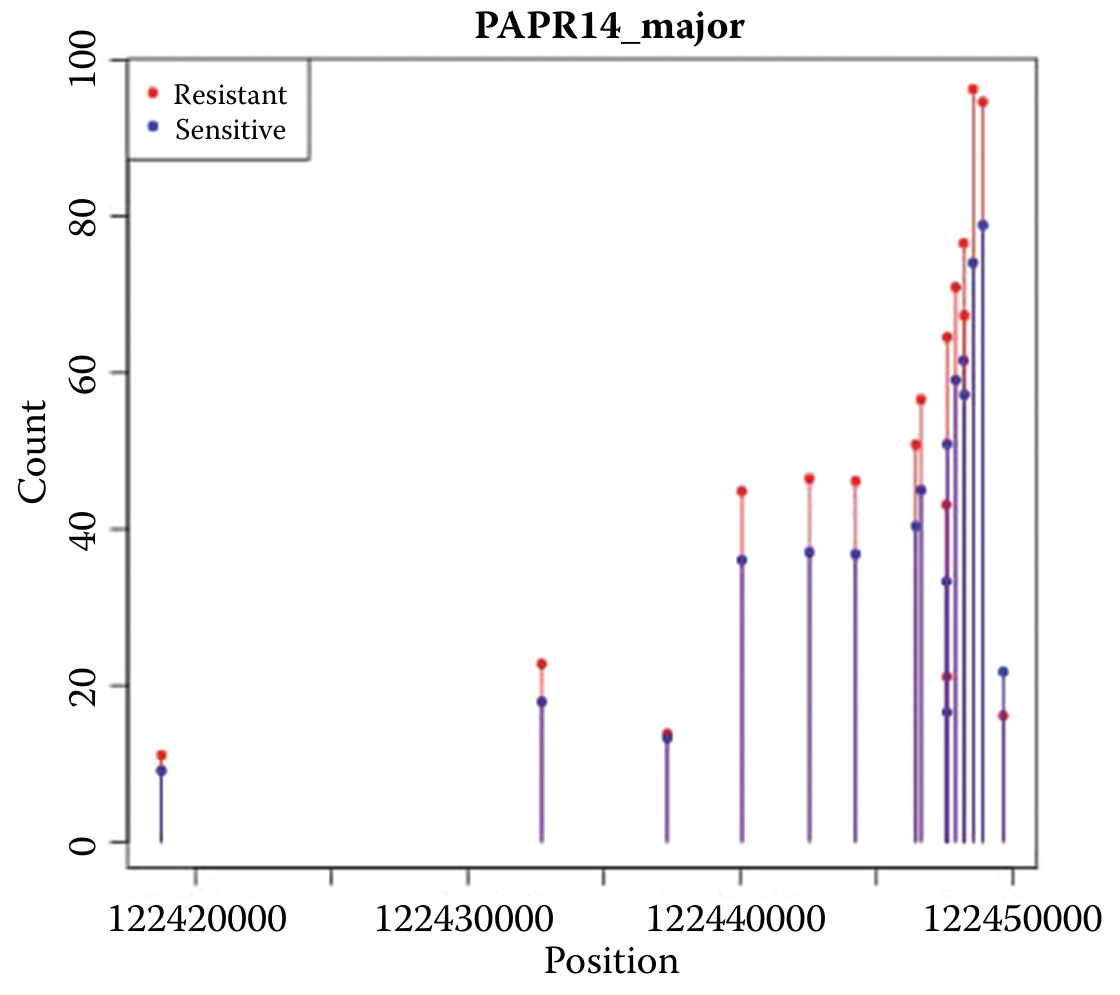
\includegraphics[width=9.8cm]{figures/ch04a_fig16_data.png}};
\fill[white] (4.7291,0.0773) rectangle (5.9744,0.4773);
\node[inner sep=0pt,fill=white,rotate=0,font=\fontsize{8}{8}\selectfont] at (5.3517,0.2773) {位置};
\fill[white] (0.1099,4.2605) rectangle (0.5099,5.2328);
\node[inner sep=0pt,fill=white,rotate=90,font=\fontsize{8}{8}\selectfont] at (0.3099,4.7467) {计数};
\fill[white] (1.4906,7.7027) rectangle (2.5383,8.0152);
\node[inner sep=0pt,fill=white,rotate=0,font=\fontsize{8}{8}\selectfont] at (2.0144,7.8590) {耐药};
\fill[white] (1.5056,7.3967) rectangle (2.5297,7.7092);
\node[inner sep=0pt,fill=white,rotate=0,font=\fontsize{8}{8}\selectfont] at (2.0176,7.5529) {敏感};
\fill[white] (4.1214,8.2613) rectangle (6.5451,8.6613);
\node[inner sep=0pt,fill=white,rotate=0,font=\fontsize{8}{8}\selectfont] at (5.3333,8.4613) {PAPR14：主要等位基因};
\end{tikzpicture}
\origfig{16}{基因 PAPR14 主要等位基因的差异表达。}
\label{fig:ch04a-16}
\end{figure}
